\documentclass{report}
\usepackage[utf8]{inputenc}
\usepackage[T1]{fontenc}
\usepackage{longtable}
\usepackage{graphicx}
 \usepackage{array}
 \usepackage{caption}
 \usepackage{graphicx}
 \usepackage{rotating}
 \usepackage[usenames,dvipsnames]{xcolor}
\usepackage{tcolorbox}
\usepackage{tabularx}
\usepackage{array}
\usepackage{colortbl}
\usepackage{color}
\usepackage{multicol}
\tcbuselibrary{skins}
%\usepackage[italian]{babel}

%Disable all warnings issued by latex starting with "You have..."
\usepackage{silence}
\WarningFilter{latex}{You have requested package}
\pdfsuppresswarningpagegroup=1

%Bib
\usepackage[
backend=biber,
style=alphabetic,
sorting=ynt
]{biblatex}
\addbibresource{References.bib}

\usepackage{csquotes}
%\usepackage{natbib}


%Import

\usepackage{tabularx}
\usepackage{marvosym}
\usepackage{fancyvrb}
%\usepackage[usenames]{color}
\usepackage[hidelinks]{hyperref}
\usepackage{url}
\usepackage{graphicx}
\usepackage{xcolor}
\usepackage{amsmath,amsfonts,amssymb,amsthm,mathtools}
\usepackage{caption}
\usepackage{enumerate}
\usepackage{multicol}
\usepackage{subcaption}
\usepackage{float}
\usepackage{indentfirst}
\usepackage{listings}
\usepackage{tocloft}
\usepackage{ifthen}
%\usepackage[most]{tcolorbox}
\usepackage{pgfplots}
%\usepackage{Style/pgfplotsthemetol}

\pgfplotsset{compat=1.16}
\definecolor{lstgrey}{rgb}{0.94,0.95,1}
\lstset{
    language=python,
    backgroundcolor=\color{lstgrey},
    frame=single,
    rulecolor=\color{lstgrey}, % make frame "invisible"
    captionpos=t,
    tabsize=2,
    numberbychapter=false,
    showstringspaces=false,
    basicstyle=\footnotesize,
    breaklines=true,
}
%LINK CLICCABILI
\hypersetup{
    colorlinks = true,
    linkcolor = .,
    citecolor = {blue},
    linkbordercolor = {white},
    urlcolor = {blue},
}
%TABELLE TBCOLORBOX
\tcbset{
        enhanced,
        colback=red!5!white,
        boxrule=0.1pt,
        colframe=red!75!black,
        fonttitle=\bfseries
       }
       
%TAB2
\newcolumntype{Y}{>{\raggedleft\arraybackslash}X}

\tcbset{tab1/.style={fonttitle=\bfseries\large,fontupper=\normalsize\sffamily,
colback=yellow!10!white,colframe=red!75!black,colbacktitle=Salmon!40!white,
coltitle=black,center title,freelance,frame code={
\foreach \n in {north east,north west,south east,south west}
{\path [fill=red!75!black] (interior.\n) circle (3mm); };},}}

\tcbset{tab2/.style={enhanced,fonttitle=\bfseries,fontupper=\normalsize\sffamily,
colback=yellow!10!white,colframe=red!50!black,colbacktitle=Salmon!40!white,
coltitle=black,center title}}

%PATH IMMAGINI
\graphicspath{{Images/}{DrawIo/}}
\newcommand{\emailaddr}[1]{\href{mailto:#1}{\texttt{#1}}}

\newcounter{Site}
\setcounter{Site}{1}

    \title{\LARGE
        \ifthenelse{\value{Site}=1}{ 
            RELAZIONE DI PROGETTO  \\ DI \\ “APPLICAZIONI E SERVIZI WEB” \\
            \hrulefill \\
        }
        Weather Vortex \\ 
        \ifthenelse{\value{Site}=1}{ 
            \hrulefill \\
        }
    }
    \author{
        Zandoli Silvia \\ \emailaddr{silvia.zandoli2@studio.unibo.it} 
        \and 
        Tentoni Daniele \\ \emailaddr{daniele.tentoni2@studio.unibo.it}
        \and
        Lirussi Igor \\ \emailaddr{igor.lirussi@studio.unibo.it}
        \\ \\ \\ 
    }


\date{\today}


\begin{document}
\maketitle
% -*- root: ../main.tex -*-
\begin{abstract}
Il presente report contiene una descrizione dettagliata di 
tutte le fasi di sviluppo del progetto Weather Vortex per Applicazioni e Servizi Web. L'applicativo è volto a ottenere e aggregare previsioni meteo da vari provider internazionali. Tale scopo verrà raggiunto grazie allo sviluppo di un'applicazione web che si interfaccia con API esterne e dispositivi IoT. 
\end{abstract}

\tableofcontents

% CONTENUTI
    % -*- root: ../main.tex -*-

% Esporre l'obiettivo del progetto dandone una visione complessiva. Devono essere illustrate le caratteristiche salienti del progetto; deve essere chiara la distinzione tra le tecnologie usate/assemblate durante lo svolgimento dell'elaborato e il contributo tecnologico/scientifico e effettivamente apportato dal gruppo.

\chapter{Introduzione}


\section{Overview}
Weather Vortex è un progetto che nasce con l'intento di fornire all'utente un servizio per consultare e paragonare diverse previsioni meteo senza dover necessariamente consultare diversi portali o siti dedicati. L'obbiettivo verrà raggiunto mediante la creazione di una \textbf{piattaforma web} che possa, da un lato, \textbf{facilitare le decisioni dell'utente}, dall'altro \textbf{fornire un'esperienza personalizzata}.

\begin{figure}[H]
    \caption{Il logo della piattaforma}
    \label{fig:Logo}
    \centering
    
\includegraphics[width=0.5\textwidth]{Images/logo.png}
\end{figure}

\section{Problemi}
Normalmente un utente consulta in media 3 / 4 siti meteo ogni volta che vuole farsi un'idea precisa delle previsioni del tempo. Questo comporta un dispendio di tempo e risorse nel consultare più fonti, quando un aggregatore potrebbe fare tutto in automatico.

\par Talvolta un utente appassionato potrebbe progettare una propria centralina meteo da collocare in un punto preciso dove gli interessa maggiormente essere informato delle condizioni meteo della zona.

\par I principali problemi che vengono attualmente riscontrati sono i seguenti:
\begin{itemize}
    \item \textbf{Diverse Fonti:} l'utente deve consultare più fonti, non fidandosi di un singolo parere, dato che generalmente non tutti i siti dedicati concordano sui risultati.
    \item \textbf{Affidabilità:} l'utente deve tenere a mente l'affidabilità dei singoli siti e/o calcolarne approssimativamente il peso sulla base delle proprie esperienze pregresse con gli stessi.
    \item \textbf{Customizzazione:} l'utente non ha possibilità nei siti più famosi di impostare una propria centralina meteo da accompagnare alle previsioni tradizionali.
\end{itemize}
 
\section{Obiettivi}
L'obiettivo consiste nel fornire all'utente un servizio per la consultazione delle previsioni meteo che risolva o quanto meno attenui i disagi o lo stress causato dai problemi sopra descritti. 

\par Nello specifico si vogliono incontrare le esigenze di chi ne fruisce, agevolando le operazioni di:
\begin{itemize}
    \item \textbf{Osservazione delle condizioni meteo}, sia attuali che fino a 5 giorni, per una determinata località.
    \item \textbf{Registrazione di un account}, permettendo il salvataggio di preferenze su una determinata località di cui ricevere le previsioni tutti i giorni sui canali di comunicazione preferiti
    \item \textbf{Assegnazione di feedbacks} ai vari provider meteo lasciando un voto sulla precisione e correttezza delle previsioni emanate. 
    \item \textbf{Registrazione di una centralina} che permetta di avere dati personalizzati per tutti gli utenti consultatori del sito, per affinare le previsioni emanate dagli altri servizi meteo o per ricevere previsioni accurate su una specifica zona.
\end{itemize}






    % -*- root: ../main.tex -*-

% Riassumere le soluzioni presenti in letteratura inerenti al problema in esame. Per ciascuna, discutere le principali diversità o affinità rispetto al progetto presentato. Nel caso non siano presenti soluzioni direttamente comparabili a quella presentata descrivere comunque le principali tecniche note per affrontare la tematica trattata. Le soluzioni esposte devono essere corredate degli opportuni riferimenti bibliografici. Nel caso si tratti di soluzioni già operative sul mercato, devono essere indicate le fonti (online) dove poter accedere al servizio o approfondirne i contenuti.

\chapter{Stato dell'Arte}
Il topic scelto in letteratura ha ricevuto molte attenzioni per via della stessa natura delle previsioni meteo, fortemente legate al machine learning. Tuttavia per quanto riguarda l'aggregazione di esse non risultano presenti particolari ricerche.
\par Dalle informazioni che abbiamo raccolto su studi e applicazioni di idee similari alla nostra è emerso quanto segue:

\begin{itemize}

    \item \textbf{Aggregazione}: sono presenti alcuni siti similari ma offrono funzionalità molto limitate, è possibile vedere solo le previsioni odierne e non permettono di scegliere quanta fiducia dare ai diversi servizi.
    
    \begin{itemize}
    
        \item Il servizio \href{https://www.metaweather.com/it/}{Metaweather} fornisce un'aggregazione di dati molto simile a quella che vogliamo ottenere con il nostro progetto, ma la visualizzazione delle recensioni dei servizi meteo non è pubblica e non viene data la possibilità di aggiungere centraline meteo.
        
        \item Google sta progettando con successo una Deep Neural Network per predire più efficacemente le condizioni meteo combinando esclusivamente i dati delle previsioni meteo negli anni passati. Applicando poi questi algoritmi alle previsioni delle ultime ore o giorni, senza alcuna conoscenza dei modelli fisici adottati fino adesso per la previsione delle condizioni meteo, è in grado di determinare talvolta con estrema accuratezza le condizioni future fino a 8 ore: \href{https://neurohive.io/en/news/google-s-deep-neural-network-makes-detailed-weather-forecasts/}{Google's Deep Neural Network}. 
        
    \end{itemize}
    
    \item \textbf{Personalizzazione}: non sono presenti siti, se non prototipali, che permettano di registrare una centralina personale da aggiungere alle fonti per le previsioni. 
    
    \par In genere gli appassionati adottano delle soluzioni pensate appositamente per le proprie centraline, che non comunicano con altri dispositivi di altri appassionati oppure con servizi meteo esistenti. Talvolta potrebbero esserci progetti che raccolgono dati da diverse centraline, ma ciò è mirato a produrre un'unica previsione meteo incrociando i dati dalle fonti. Viene perso il riferimento ad ogni centralina e i suoi dati, producendo una previsione meteo unica per tutta la zona.
    
\end{itemize}
 


    % -*- root: ../main.tex -*-
\chapter{Processo di Sviluppo}


\section{Metodologia di Sviluppo}
Prima di iniziare a lavorare è stato fondamentale accordarsi su come affrontare in gruppo un progetto mediamente complesso come questo. Si è pensato subito di utilizzare una metodologia agile, per evitare confusioni e lavorare efficientemente in team. Si è optato quindi per la metodologia Scrum.\vspace{0.5cm}

    Scrum è una metodologia agile, incrementale e iterativa per lo sviluppo di prodotti, applicazioni e servizi. E' una modalità strutturata e pianificata.\\
    Scrum si basa sull’empirismo, ovvero sul concetto che la conoscenza derivi dall’esperienza e che le decisioni vadano prese alla luce di ciò che si conosce. I tre pilastri che sostengono l’empirismo sono: trasparenza, ispezione e adattamento.\\
    Ovvero, tutti gli aspetti del lavoro devono essere visibili ai responsabili del risultato finale (trasparenza). Per rendere trasparenti questi elementi, il Team Scrum ispeziona di frequente il prodotto mentre lo sta sviluppando (ispezione). Così il processo e il prodotto possono essere adattati immediatamente nel caso di nuove esigenze o di condizioni mutate del mercato (adattamento).\\ 
    Perchè questo è il senso di Scrum, far lavorare tutto il team insieme, in modo coordinato e organizzato.\\
    Come tutte le metodologie Agile, si basa sulla divisione del progetto in più fasi, chiamate Sprint.\\
Ad ogni Sprint il gruppo di lavoro presenta nuove funzionalità, operative e implementabili. Si configura così un sistema iterativo che consente di incrementare poco alla volta, ma molto di frequente, le funzionalità del progetto, verificando costantemente allo stesso tempo l'andamento complessivo.\vspace{0.5cm}

Siamo sempre stati fedeli nell'utilizzare tale metodologia, ma durante il progetto spesso è stata cambiata la durata degli Sprint, per il semplice fatto che per vari motivi non si riusciva a portare a termine i compiti assegnati entro la settimana. Il risultato è stato sicuramente l'allungamento dei tempi nella realizzazione del progetto, ma non abbiamo mai smesso di seguire tale metodo di lavoro e di confrontarci.

\section{Gestione di Progetto}
In questa sezione viene dettagliatamente spiegato come il progetto è stato organizzato. Gli strumenti e tecnologie con cui è scelto di procedere verranno elencati assieme alla descrizione della metodologia.
    \paragraph{Come ci siamo organizzati}
    Nel nostro caso abbiamo suddiviso il lavoro in Sprint che avevano durata di una settimana. Ad ogni Sprint corrispondevano diverse attività o issue, che di solito venivano assegnate ad ognuno di noi a inizio settimana. Esse dovevano essere completate la settimana seguente.
    
    \paragraph{Gantt Chart} 
    A partire da inizio progetto abbiamo stilato un diagramma di Gantt, uno strumento utile per la pianificazione dei progetti. Attraverso una panoramica dei compiti programmati, ci ha permesso di venire a conoscenza dei compiti e delle rispettive scadenze.
    
    
    \paragraph{Licensing} Per quanto riguarda la gestione delle licenze, è stato scelta, tra le varie disponibili, 
    
    \paragraph{Versioning}
    Per il versioning ci siamo avvalsi di Github. 
    
    \paragraph{GitHub Projects Management}
    descrizione GitHub Projects boards 
    
    \paragraph{Telegram}
    Abbiamo creato un gruppo Telegram per aggiornarci giornalmente sullo sviluppo del progetto, esprimere eventuali dubbi e avere ulteriori chiarimenti. 
    
    \paragraph{Incontri}
    Abbiamo deciso di sentirci una volta a settimana, per risolvere insieme alcuni task rimasti, fare il chiarimento della situazione e stilare lo Sprint per la settimana successiva. Abbiamo alternato sia sedute in presenza che online, dove ci siamo avvalsi della piattaforma Microsoft Teams.
    
     

\section{Continuous Integration e Automatizzazione}
\label{chap:CI}
In questo capitolo si analizza la parte di integrazione e automatizzazione sia del progetto software che della relazione. 
    \subsection{Relazione di Progetto}
        descrizione CI della relazione da Overleaf a GitHub action e la release

    \subsection{Progetto}
        CI implementata per il testing 
        
        






    % -*- root: ../main.tex -*-

% In questa sezione esporre brevemente i requisiti a cui il sistema proposto deve rispondere, concentrando l'attenzione sugli aspetti più rilevanti e facendo eventualmente uso di opportuni diagrammi di alto livello.

\chapter{Analisi dei Requisiti}
In questa fase sono stati individuati i \textbf{requisiti del sistema}, partendo dalle descrizioni di alto livello, ottenute dal committente durante il \textbf{knowledge crunching e i focus group}. Successivamente si è proceduto con un raffinamento che ha portato alla definizione di requisiti più \textbf{specifici}, \textbf{chiari} e \textbf{strutturati}.
	
	\section{Requisiti di Business}
	Si definiscono di seguito le aspettative del cliente e i requisiti che il prodotto dovrà soddisfare, espressi con una terminologia ad elevato livello astrattivo.
        \begin{itemize}
            \item L'applicativo dovrà \textbf{ridurre il tempo necessario} per consultare più previsioni.
            \item Il prodotto dovrà ...
            \item Opzionalmente il prodotto dovrà \textbf{...} 
        \end{itemize}
	
	\section{Requisiti Utente}
	Di seguito vengono riportate le richieste mosse dal cliente in maniera informale evitando termini tecnici, successivamente tali richieste saranno formalizzate per quanto possibile.
	Il prodotto dovrà fornire: 
		\begin{itemize}
            \item l'accesso al sistema da \textbf{qualunque dispositivo} munito di connessione alla rete, anche mobile o tablet
            \item \textbf{prestazioni adeguate} per il caricamento
            \item un interfaccia intuitiva
            \item account
            \item possibilità di registrare una centralina
        \end{itemize}
        \subsection{User stories}
        Di seguito sono riportate tutte le \textbf{user stories} formulate assieme agli utilizzatori
        \begin{itemize}
            \item Come \textbf{utente}
            voglio:
            \begin{itemize}
                \item poter \textbf{visualizzare} le previsioni odierne
                \item poter \textbf{visualizzare} le previsioni relative ai prossimi giorni
                \item voglio poter \textbf{impostare} la fiducia per ogni servizio usato
                \item poter \textbf{aggiungere un device} 
                
            \end{itemize}
        \end{itemize}
            
	    
	\section{Requisiti Funzionali} %obbligatori, desiderabili e opzionali
	Di seguito si riportano i requisiti non funzionali:
	    \subsection{Casi d'uso}
        	 Diagramma dei casi d'uso
                    
        \subsection{Applicativo web}
        L'applicativo web deve consentire ad ogni utente di accedere con una serie di credenziali, e dividere le operazioni consentite in base ai permessi concessi.
        Il sito è suddiviso pagine :
        \begin{itemize}
            \item \textbf{pagina di login}
                La pagina utilizzata per effettuare l'accesso
            \item \textbf{home}
                La pagina principale in cui è possibile:
                \begin{itemize}
                    \item accedere
                    \item registrarsi
                    \item consultare le previsioni
                \end{itemize}
            
        \end{itemize}
        
    
        
	\section{Requisiti non Funzionali}	
    Il sistema dovrà rispettare i seguenti requisiti non funzionali per un'alta \textbf{qualità}:
        \subsection{Di Sistema}
            \begin{itemize}
                \item \textbf{Reattività}: 
                    \begin{itemize}
                        \item l'utente non deve percepire \textbf{ritardi} 
                        \item le notifiche devono ..
                    \end{itemize}
                \item \textbf{Scalabilità}: L'applicativo deve necessariamente consentire di aumentare o diminuire il numero di utenti gestiti senza particolari problemi. 
            \end{itemize}
        

	\section{Requisiti Implementativi}
	Si definiscono i vincoli a livello tecnologico e di implementazione che sarà necessario rispettare nella realizzazione dell'applicativo.
	
	\subsection{Metodologie e Tecnologie Utilizzate}
	In quanto progetto sviluppato per l'esame di Applicazioni e Servizi Web è necessario che le tecnologie usate rispettino gli standard di insegnamento. 
	
    % -*- root: ../main.tex -*-

% Devono essere esposte le scelte progettuali operate nelle varie fasi di sviluppo dell'elaborato. In questa sezione devono essere documentati gli schemi di progetto relativamente all'architettura complessiva del sistema e alle sue componenti di rilievo che possano meritare un'analisi di dettaglio. Per le componenti software si può ricorrere ad esempio a diagrammi delle classi, di sequenza, stato, attività. Per le componenti hardware è possibile includere opportuni schemi in grado di descrivere l'architettura fisica adottata.

\chapter{Design Architetturale}

    \section{Architettura Generale}
    
    Abbiamo deciso di dividere il nostro sistema in due macro componenti: un applicativo server, che si occupi di gestire le richieste degli utenti, e un applicativo client, che si occupi di interrogare il server per richiedere informazioni. Le specifiche imposte dalla prova di esame in corso imponevano di usare determinate tecnologie per lo sviluppo di tali componenti, ma non imponevano altri vincoli. Abbiamo scelto noi di sviluppare i due componenti come progetti separati per aumentare l'indipendenza di un componente rispetto l'altro.
    
    \par Le funzioni da qui demandate all'applicativo \textbf{Server} sono:
    
    \begin{itemize}
    
        \item Richiesta di previsioni meteo da providers esterni: ci siamo registrati ai seguenti provider di previsioni meteo internazionali:
        
        \begin{itemize}
            
            \item Open Weather Map
            \item Troposphere
        
        \end{itemize}
        
        Quando il server viene interrogato per una previsione, la richiede a sua volta alle sorgenti di dati disponibili, che possono essere:
        
        \begin{itemize}
            \item Servizi esterni (sopra citati)
            \item Centraline degli utenti registrati
        \end{itemize}
        
        Non appena i risultati saranno ricevuti, sono immediatamente processati e forniti in output. Le unità di misura devono essere tutte uniformi e convertite all'occorrenza.
        
        \item Richiesta di autenticazione da parte dei client: date le credenziali degli utenti, il server si deve occupare di verificarne la presenza nella base dati degli utenti registrati nel sito. Dopo averne verificato l'autenticità e la validità, deve rilasciare un token di autenticazione da utilizzare nel caso in cui bisognasse richiedere delle risorse protette.
        
        \item Richiesta di feedbacks dei providers meteo: fornire un sistema di recensioni, le quali possono essere lasciate per ogni provider in base alla correttezza delle sue previsioni meteo. Successivamente calcolare la valutazione media di ogni servizio consultabile.
        
        \item Notifica di previsioni meteo a caselle di posta elettronica: configurando un account di posta elettronica per il proprio utente, il server deve poter inviare delle emails a chi ne fa richiesta per poter conoscere, all'inizio della propria giornata o nel momento che si ritiene più opportuno, le previsioni per la località preferita.
        
    \end{itemize}
    
    \par Le funzioni da qui demandate all'applicativo \textbf{Client} sono:
    
    \begin{itemize}
    
        \item Presentazione del progetto, degli autori e delle funzionalità messe a disposizione.
        
        \item Fornitura di un'interfaccia utente semplificata per la richiesta delle previsioni meteo all'applicativo Server:
        
        \begin{itemize}
            \item che renda comodo ed intuitivo la consultazione e la fruizione delle previsioni meteo dei vari providers
            
            \item che calcoli in automatico le statistiche relative alla distribuzione, alle differenze e similitudini dei risultati ottenuti dalle api
        \end{itemize}
        
        \item Gestione delle impostazioni e dei dati personali degli utenti: registrandosi al sito, ogni utente fornisce un insieme di dati e informazioni che devono essere mantenute, consultabili e modificabili agilmente. Le informazioni gestite comprendono anche la località preferita dell'utente, le centraline registrate e i feedbacks rilasciati.
        
        \item Gestione dei feedbacks rilasciati dagli utenti: deve rendere possibile creare delle recensioni per i providers e renderle consultabili da tutti gli utenti, assieme alla valutazione media del servizio stesso.
    
    \end{itemize}
    
    \par Oltre a questi componenti deve essere sviluppato anche il componente per simulare una centralina meteo amatoriale che possa ricevere le richieste del server per ottenere le previsioni meteo della zona in cui è situata. Per fare questo, abbiamo creato un nuovo progetto indipendente che assolva a questi compiti.

    \begin{figure}[H]
        \caption{Architettura Generale}
        \label{fig:General}
        \centering
        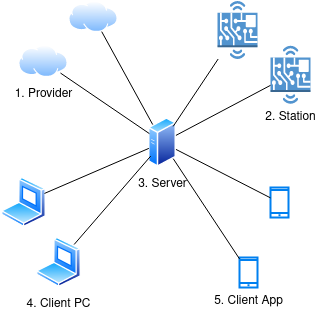
\includegraphics[width=0.5\textwidth]{DrawIo/General.png}
    \end{figure}
    
    \par Nel seguente schema vengono anche mostrati altri due componenti, chiamati Providers, che rappresentano i servizi esterni a cui ci affidiamo per ottenere dei dati meteo veritieri.
    
    \section{Scelte Tecnologiche Cruciali}
    
    Avendo l'esigenza di fornire all'utente i risultati delle previsioni meteo da lui richieste non appena essi fossero stati pronti, una scelta cruciale per il progetto è stata scegliere riuscire una tecnologia per mantenere un canale dati aperto tra il Client e il Server. Il protocollo HTTP non fornisce di per se un meccanismo tale per cui sia il Server ad inviare una richiesta di connessione al Client. Per questo motivo si è optato ad un approccio basato sulle Sockets. In particolare, abbiamo scelto la libreria \textit{Sockets.IO}, già vista a lezione.

    \section{Pattern Architetturali Utilizzati}
    
        
    
        \subsection{Client-Server}
        
            Nella figura 5.2 è illustrato come avviene un flusso di richieste di previsioni meteo dal Client al Server.
        
            \begin{figure}[H]
            
                \caption{Diagramma delle attività di una richiesta di previsioni dal Client al Server}
                
                \label{fig:Forecast Request Activity Diagram}
                
                \centering
                
                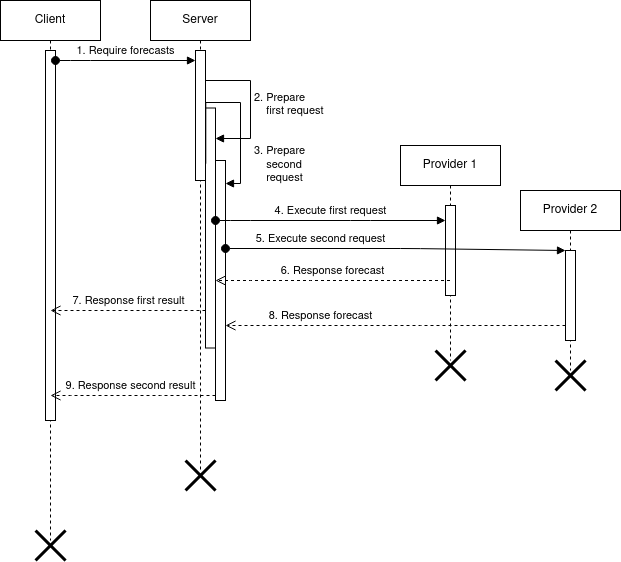
\includegraphics[width=0.75\textwidth]{DrawIo/forecast_request_activity_diagram.png}
                
            \end{figure}
            
            Procedendo in ordine numerico, al punto 1., il Client invia una richiesta al Server contenente il nome della località di cui vuole sapere le coordinate. Il Server nei punti 2. e 3. prepara la richiesta da inviare ai vari provider di previsioni meteo. Nello specifico vengono preparate solamente altre due richieste per altrettanti providers, ma in un caso reale potrebbero essercene molte di più. Da notare come in questo punto avvenga una divisione del flusso computazionale principale in due flussi separati ed indipendenti. Nei punti 4. e 5. tali flussi eseguono autonomamente le richieste delle previsioni al provider meteo esterno a loro assegnato. Ricevuta la risposta nei punti 6. e 7., la inoltrano al Client nei punti 7. e 8..
    % -*- root: ../main.tex -*-
\chapter{Design di Dettaglio}
In questo capitolo verrà spiegato come si è giunti a realizzare l’applicativo,
confrontando poi i mockup con le effettive interfacce utente, descrivendone i componenti e infine mostrando lo schema della base di dati implementata.

Come tutti i programmi, il progetto è costituito da  frontend e backend.
Questi denotano rispettivamente la parte visibile all'utente di un programma e con cui egli può interagire —tipicamente un'interfaccia utente— e la parte che permette l'effettivo funzionamento di queste interazioni. \newline
Il frontend, nella sua accezione più generale, è responsabile dell'acquisizione dei dati di ingresso e della loro elaborazione con modalità conformi a specifiche predefinite e invarianti, tali da renderli utilizzabili dal backend. Il collegamento del frontend al backend è un caso particolare di interfaccia.

\section{Frontend}
Fin dall'analisi del progetto è stato chiaro che il target dell'applicazione fosse ampio, infatti l'insieme degli utenti interessati comprende chiunque abbia la
necessità di consultare delle previsioni meteo.
Per questo motivo, le interfacce e il funzionamento dell'applicazione sono stati progettati per essere adoperati anche dagli utenti meno esperti.

\subsection{Interfacce utente}
In seguito ad un'analisi preliminare del problema sono stati prodotti dei mockup della grafica per dare l'idea delle funzioni e dei requisiti dell'applicativo. 
Le pagine effettive si sono evolute durante lo sviluppo ma mantengono le linee guida dei mockup. 
Vengono descritte le interfacce utente più importanti.
Si consulti anche il capitolo \ref{prodottofinale} per visualizzare il risultato finale delle pagine.

\begin{figure}[H]
    \caption{Home}
    \label{fig:Home}
    \centering
    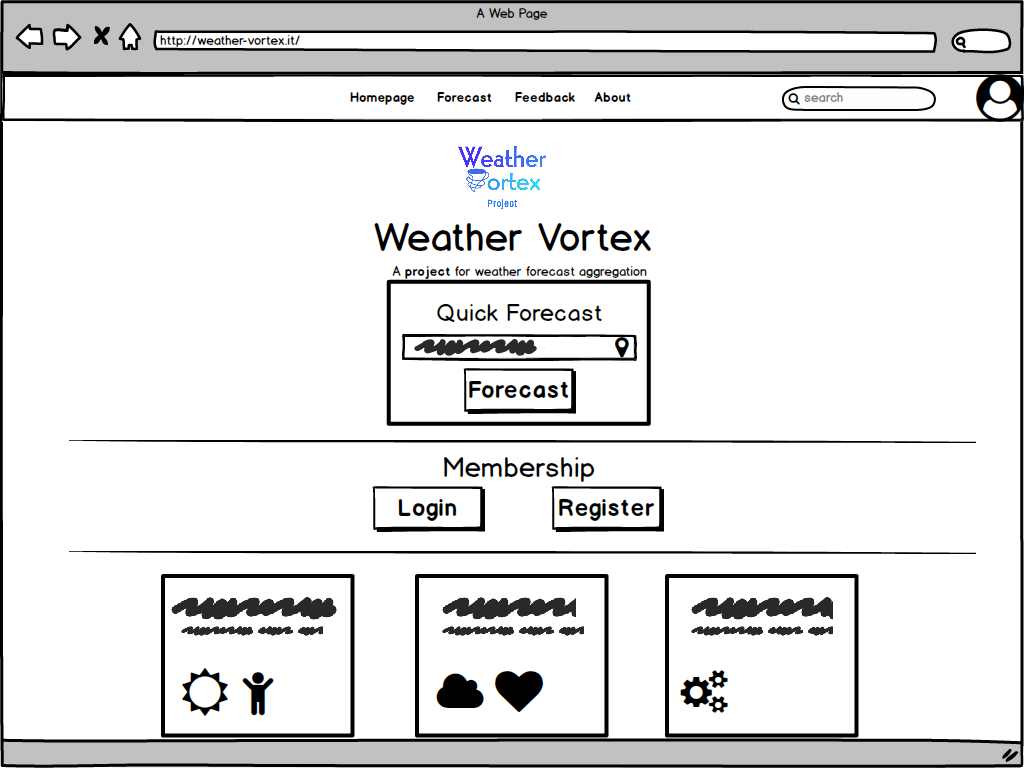
\includegraphics[width=0.6\textwidth]{MockUps/homepage.png}
\end{figure}
La homepage è la pagina principale di presentazione.
In bella vista presenta una card con una barra di testo dove inserire il nome della località con l'icona di una mappa per le coordinate geografiche, con due bottoni in basso per richiedere le previsioni. 
Attraverso i bottoni Login e Register inoltre si può accedere alle pagine di autenticazione.

\begin{figure}[H]
    \caption{Login}
    \label{fig:Login}
    \centering
    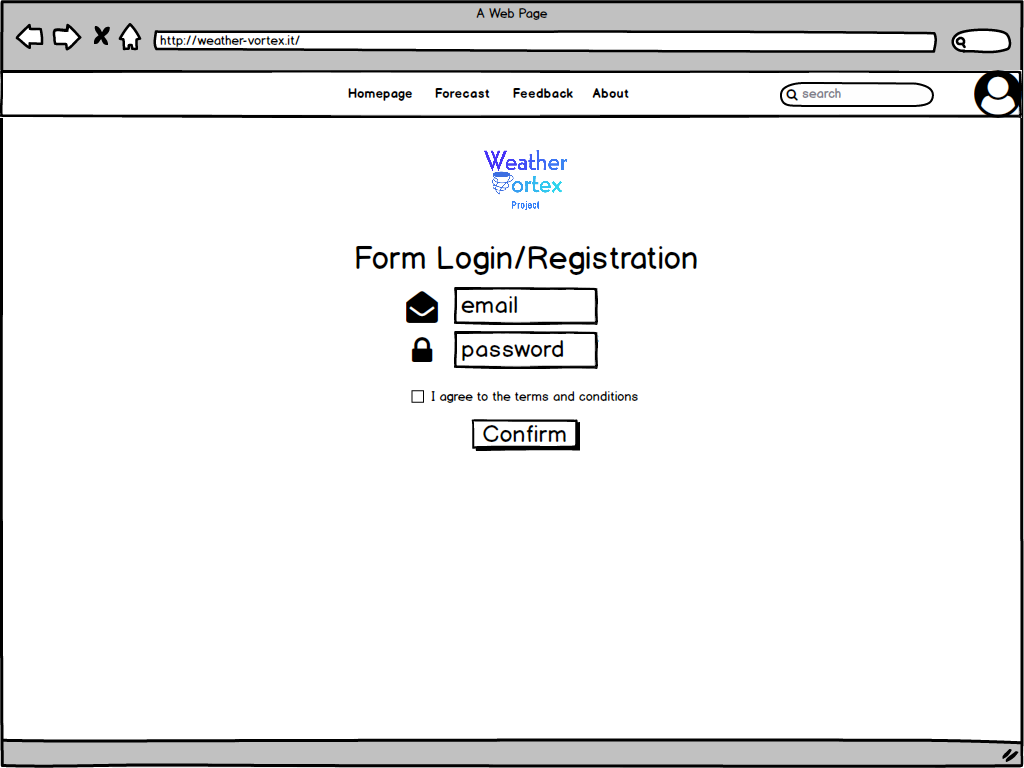
\includegraphics[width=0.6\textwidth]{MockUps/Login_Register.png}
\end{figure}
Viene pensata una pagina di login classica con la possibilità di recuperare la password e una pagina di registrazione. Effettuata la registrazione viene chiesto agli utenti di completare la propria iscrizione cliccando sul link dell'email di conferma.

\begin{figure}[H]
    \caption{Forecast}
    \label{fig:Forecast}
    \centering
    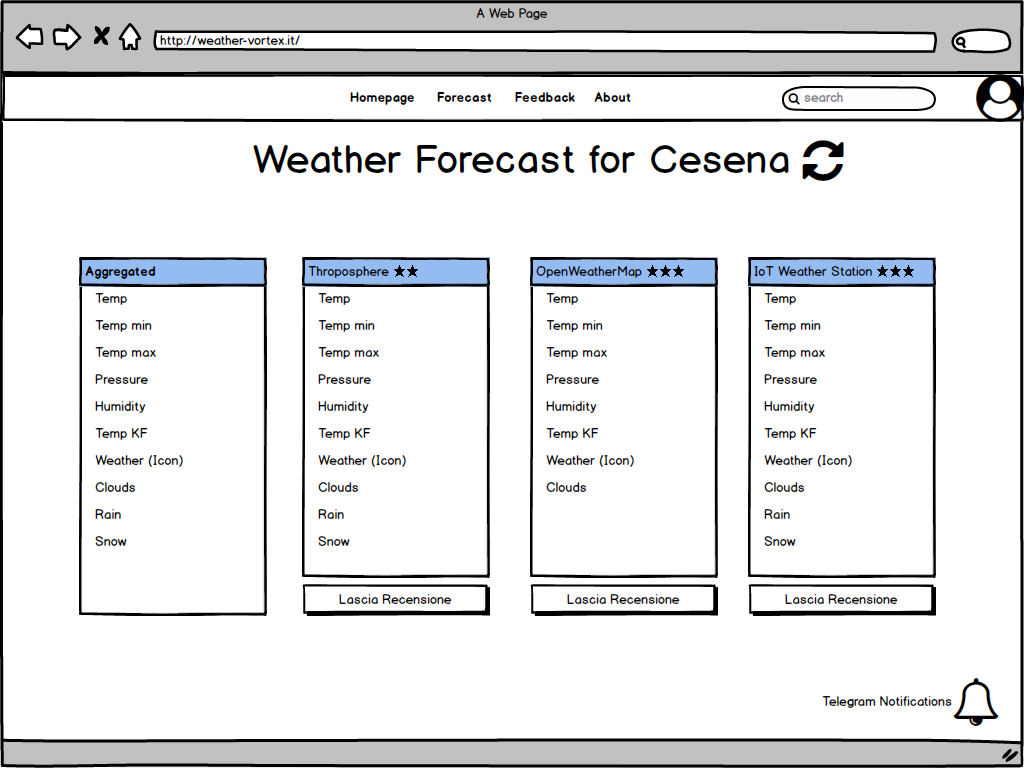
\includegraphics[width=0.6\textwidth]{MockUps/forecast.png}
\end{figure}
Il fulcro dell'applicazione è sicuramente la pagina delle previsioni. Inizialmente la pagina visualizza un'immagine esplicativa con in alto una barra di testo dove inserire la località oppure richiedere le coordinate geografiche attuali attraverso l'icona della mappa. Cliccando sui due pulsanti a lato si può richiedere il meteo attuale o quello dei prossimi tre giorni. Comparirà così in posizione centrale la card della previsione aggregata e in basso un insieme di schede che rappresentano le previsioni di ogni provider, con informazioni utili sul meteo.
 Nel caso siano richieste le previsioni dei prossimi tre giorni, la pagina si aggiornerà mettendo a disposizione un tooltip di bottoni per scegliere il giorno specifico e uno slider per scegliere l'ora della previsione.

\begin{figure}[H]
    \caption{Feedbacks}
    \label{fig:Feedbacks}
    \centering
    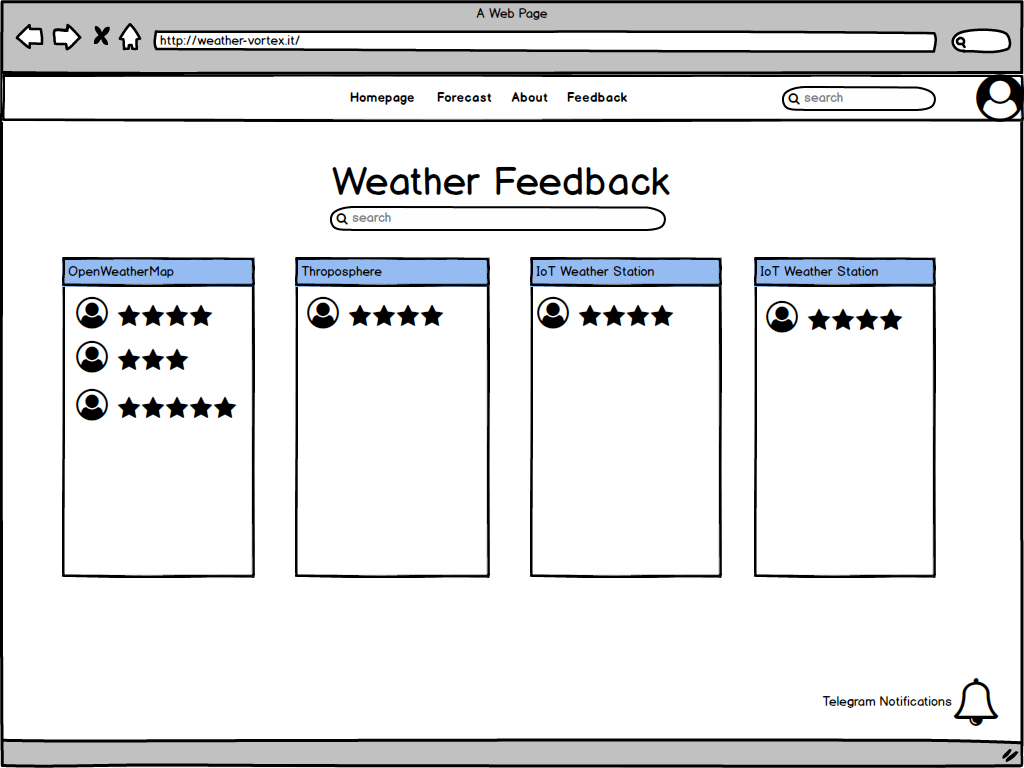
\includegraphics[width=0.6\textwidth]{MockUps/feedback.png}
\end{figure}
Nella pagina delle recensioni è possibile visualizzare uno slider che contiene le schede con le recensioni relative ai vari provider. Tramite la barra di ricerca in alto è possibile trovare quello desiderato digitandone parte del nome. Ogni scheda contiene una lista di recensioni lasciate dagli utenti. Per ogni recensione viene mostrato l'avatar dell'utente che l'ha rilasciata, con a lato la sua valutazione. Questa è stata espressa graficamente da una a cinque stelle. Cliccando sul campo è possibile visualizzare il profilo pubblico dell'utente associato.

\begin{figure}[H]
    \caption{Aggiunta di una recensione}
    \label{fig:FeedbacksDialog}
    \centering
    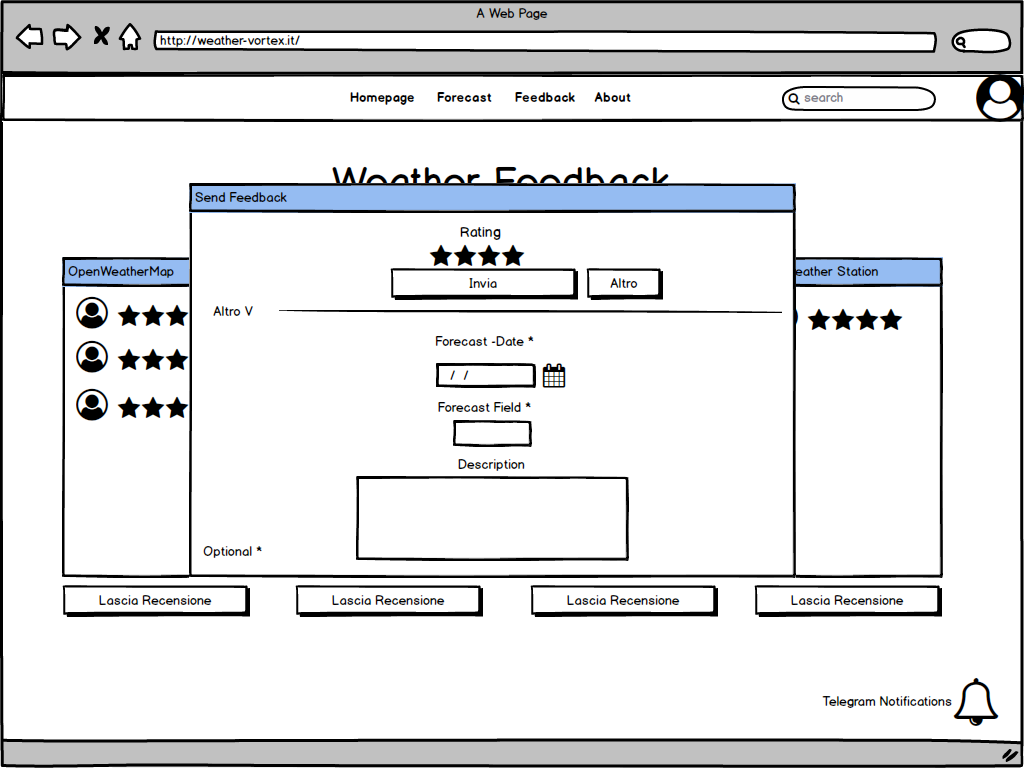
\includegraphics[width=0.6\textwidth]{MockUps/sendFeedback.png}
\end{figure}

All'estremità di ogni scheda, se si è autenticati, sarà presente il pulsante per aggiungere una nuova recensione. Se si clicca su di esso si visualizzerà una finestra con il rating da inserire. Questa è espandibile: si possono anche specificare il campo della previsione che si vuole recensire (ad esempio temperatura minima, Pressione, etc), la data della previsione alla quale ci si riferisce, e eventuali note.
In cima ad ogni card si è deciso di far visualizzare una statistica, calcolata come media dei rating di quel provider. Si tratta di un indice di affidabilità che calcola l'accuratezza della previsione, basandosi sull'opinione delle altre persone.

\begin{figure}[H]
    \caption{Private Profile}
    \label{fig:PrivateProfile}
    \centering
    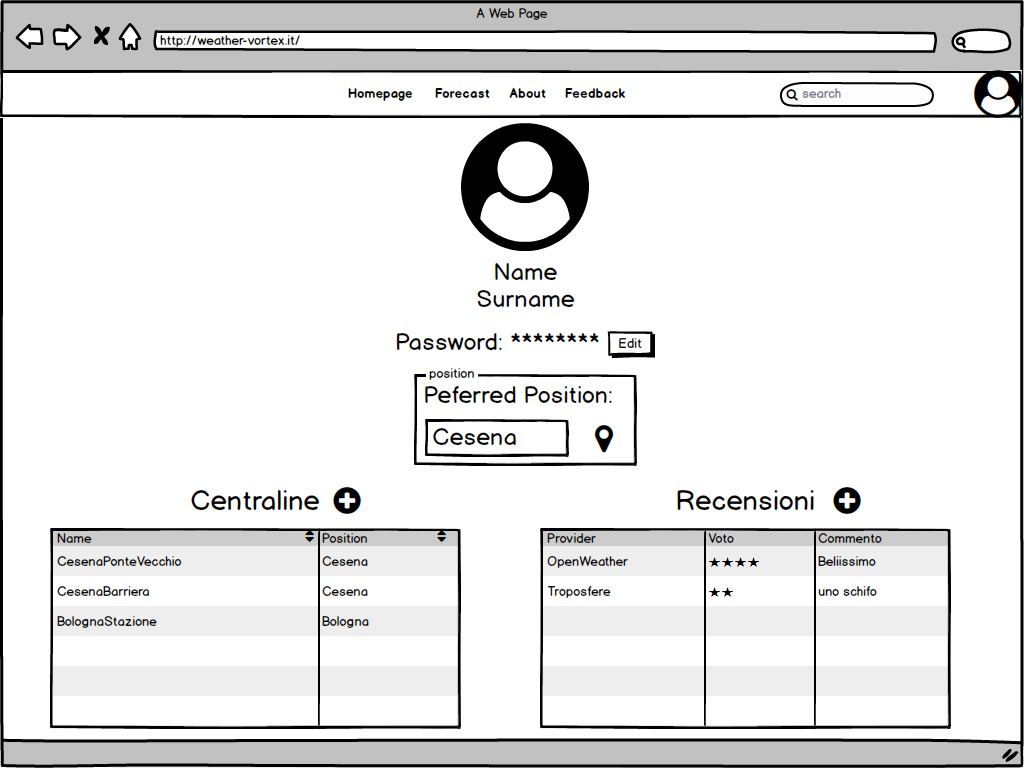
\includegraphics[width=0.6\textwidth]{MockUps/Private Profile.png}
\end{figure}
La pagina del profilo privato dà la possibilità ad ogni utente di visualizzare e gestire le proprie informazioni personali. Cliccando su "edit" si aprirà un dialog che consentirà di poter modificare la propria password o la propria posizione preferita.
L'utente ha la possibilità di visualizzare le proprie centraline, di aggiungerle tramite il pulsante "+" in alto della tabella, modificarle e eventualmente cancellarle (ne verrà richiesta la conferma).
L'utente ha la possibilità di visualizzare le proprie recensioni e eventualmente cancellarle (ne verrà richiesta la conferma).
Navigando in questa pagina c'è anche la possibilità di cancellare il proprio account tramite un bottone apposito in fondo alla pagina.

La pagina del Profilo pubblico ha la stessa struttura del Profilo privato, ma qui nessuna operazione di modifica è concessa.

\begin{figure}[H]
    \caption{About}
    \label{fig:About}
    \centering
    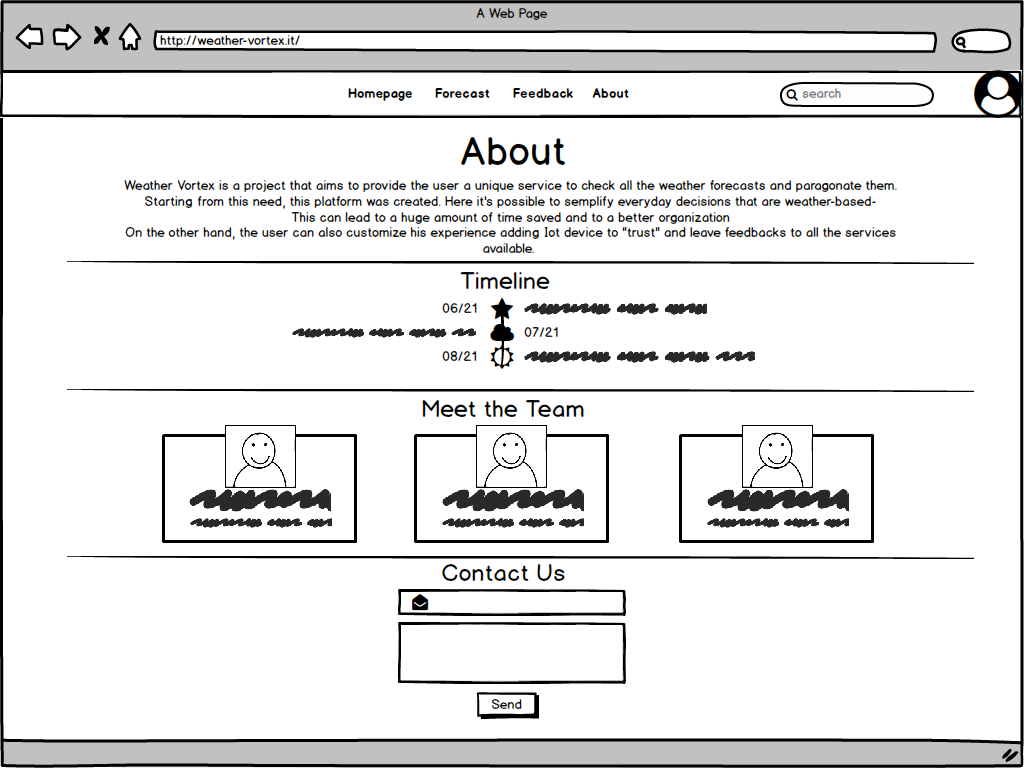
\includegraphics[width=0.6\textwidth]{MockUps/about.png}
\end{figure}
Infine una pagina per i contatti che consente l'inserimento di un messaggio/ticket
per il supporto tecnico e alcune informazioni sul team di sviluppo.

\subsection{Componenti}
Si descrivono in breve i componenti principali usati per ogni pagina.
Prima di tutto si elencano i componenti presenti in tutte le pagine:
\begin{itemize}
    \item Appbar:  E' una barra colorata situata nella zona alta della pagina. Contiene tre componenti:
    \begin{itemize}
    \item Icona Utente: Situata nell'estremità destra, permette di autenticarsi o registrarsi al sito se l'utente non ha eseguito l'accesso, altrimenti esso può visualizzare la propria pagina del profilo privato o effettuare il logout. Il suo aspetto cambia: se è autenticato mostra le iniziali del proprio nome e cognome, altrimenti mostra un'icona generica. 
    \item Titolo Weather Vortex: Situata nella parte centrale, permette di navigare alla home cliccando su di esso.
    \item Icona Menù: Situata nell'estremità sinistra, consente di mostrare o nascondere la barra di navigazione (Navbar).
    \end{itemize}
    \item Navbar: Si tratta della barra di navigazione attraverso cui l'utente può muoversi nelle principali finestre del sito.
    \item Footer: Il footer a fine pagina contenente dei link utili.
\end{itemize}
La pagina Home è composta dai principali componenti:
\begin{itemize}
    \item QuickForecastCard: Card che viene usata come scorciatoia per visualizzare le previsioni. 
    \item AccountButtons: Contiene i bottoni per accedere alle pagine di autenticazione.
    \item InfoMain: Insieme di cards di descrizione
    \item checkStatus: Card che mostra lo stato del server.
\end{itemize}
La pagina Feedbacks è composta dai seguenti componenti:
\begin{itemize}
    \item SlidesOrizontalGroup: Si tratta dello slider che contiene le schede dei vari provider con le recensioni. E' composto da due sottocomponenti:
    \begin{itemize}
        \item ServiceRatingList: Rappresenta la lista delle recensioni del provider. Ogni campo recensione è composto dall'avatar dell'utente, dalle sue iniziali e dalla sua recensione.
        \item FeedbackDialog: Rappresenta il dialog per l'aggiunta della recensione.
    \end{itemize}
\end{itemize}
La pagina Forecast è composta dai seguenti componenti:
\begin{itemize}
    \item EmptyForecast: Mostra la pagina iniziale delle previsioni.
    \item CurrentForecast: Mostra la pagina del meteo attuale. E' composta dal seguente sottocomponente: 
    \begin{itemize}
    \item ForecastGroup. Esso rappresenta l'insieme delle previsioni meteo. Richiama il componente WeatherForecastCard che rappresenta una singola previsione per uno specifico provider o il meteo aggregato. Esso contiene la descrizione del meteo, la data, la temperatura minima e massima, la pressione, l'umidità, la quantità di nuvole, di pioggia e di neve. 
    \end{itemize}
    \item ThreeDaysForecast: Mostra la pagina delle previsioni dei prossimi tre giorni. Richiama gli stessi componenti di "CurrentForecast".
\end{itemize}
La pagina Profilo Privato è composta dai seguenti componenti:
\begin{itemize}
    \item PrivateUserCard: Si tratta della card che visualizza le informazioni private dell'utente: avatar, nome, cognome, data di creazione, email, posizione preferita e bottone di modifica.
    \item PrivateUserReviews: Tabella che visualizza le recensioni rilasciate. Contiene i relativi campi: provider, valutazione, commento e un pulsante per la cancellazione.
    \item PrivateUserControlUnits: Tabella che visualizza tutte le centraline inserite. E' costituita dai seguenti campi: nome, posizione, url e due pulsanti per la modifica e la cancellazione.

\end{itemize}
La pagina Profilo Pubblico ha i seguenti sottocomponenti:
\begin{itemize}
    \item PublicUserCard: Si tratta della card che visualizza le informazioni pubbliche dell'utente: avatar, nome, cognome, eventuale posizione preferita.
    \item PublicUserReviews: Tabella che mostra le recensioni lasciate dall'utente. Contiene i seguenti campi: provider, recensione, commento.
    \item PublicUserControlUnits: Tabella che visualizza tutte le centraline inserite dell'utente. E' costituita dai seguenti campi: nome, posizione, url.

\end{itemize}   
La pagina About è composta dai seguenti componenti:
\begin{itemize}
    \item Timeline: Componente che visualizza cronologicamente gli vari stadi del progetto.
    \item MeetTeam: Un insieme di cards per descrivere gli autori del progetto. 
    \item ContactUs: Componente che funge da modulo di contatto.
\end{itemize}
\subsection{Vue-Router}
Oltre ai componenti descritti sopra all'interno di ogni pagina un componente di Vue.js che è stato utilizzato è il vue-router, per il routing e la navigazione delle pagine.
Esso consente, tramite una router-view, di visualizzare i componenti
desiderati (che insieme compongono le varie interfacce utente).
\section{Backend}
Viene ora mostrato lo schema di database utilizzato dall'applicazione:
\begin{figure}[H]
    \caption{Database}
    \label{fig:Database}
    \centering
    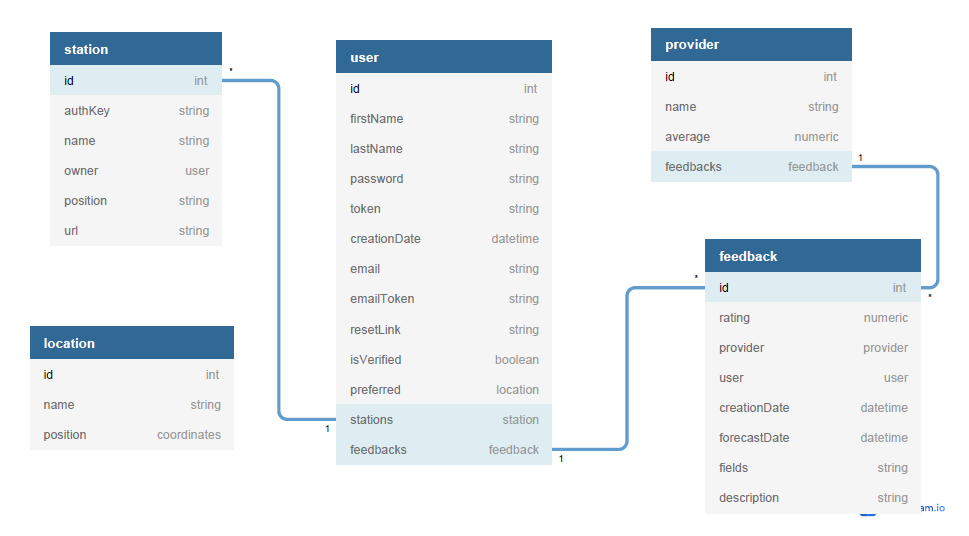
\includegraphics[width=1.0\textwidth]{DrawIo/database.png}
\end{figure}
\subsection{Modelli}
Ci sono cinque modelli
che sono il fulcro dell'applicazione, essi si trovano nella cartella models. Essi costituiscono un modello di dati da salvare in MongoDB, che vengono usati per istanziare oggetti che saranno automaticamente dotati di metodi per svolgere le classiche operazioni CRUD.
\begin{itemize}
\item user - Rappresenta il modello dell'utente. I suoi campi sono:
\begin{itemize}
\item firstName: nome dell'iscritto.
\item lastName: cognome dell'iscritto.
\item password: password dell'iscritto.
\item email: email dell'iscritto.
\item token: stringa generata durante il login per verificare l'autenticazione dell'utente.
\item creationDate: data di creazione dell'account.
\item emailToken: token per verificare l'iscrizione.
\item resetLink: token per il cambio della password.
\item isVerified: booleano che indica se l'utente è stato verificato.
\item preferred: una eventuale località preferita.
\item stations: elenco delle centraline dell'utente.
\item feedbacks: elenco delle recensioni dell'utente.
\end{itemize}
\item feedback - Rappresenta il modello della recensione. I suoi campi sono: 
\begin{itemize}
    \item rating: valutazione della recensione. 
    \item provider: il provider a cui la recensione si riferisce.
    \item user: utente che ha rilasciato la recensione.
    \item creationData: data di creazione della recensione.
    \item forecastData: data della previsione su cui si è basata la valutazione della recensione.
    \item fields: eventuali campi della previsione da valutare.
    \item description: eventuale descrizione.
\end{itemize}
\item location - Rappresenta il modello della località. I suoi campi sono:
\begin{itemize}
    \item name: nome della località.
    \item position: posizione della località espressa in coordinate geografiche tramite latitudine e longitudine.
\end{itemize}
Serve per memorizzare le richieste di previsioni che sono state fatte.
\item provider - Rappresenta il modello del provider che fornisce il meteo. I suoi campi sono:
\begin{itemize}
    \item name: nome del provider.
    \item average: la media di tutte le valutazioni date al provider.
    \item feedbacks: lista di tutte le recensioni del provider date dagli utenti.
\end{itemize}
\item station - Rappresenta  il modello della centralina. I suoi campi sono:
\begin{itemize}
    \item authKey: valore usato per autenticare richieste alla stazione.
    \item name: nome della centralina.
    \item owner: proprietario della centralina.
    \item position: nome della località in cui si trova.
    \item url: url della centralina.
\end{itemize}
\end{itemize}
\subsection{Storage}
Gli storage sono dei componenti che si occupano di manipolare i dati e i modelli dell'applicazione nascondendo il supporto di memorizzazione degli stessi. 
\begin{itemize}
\item{database storage} - storage che usa come supporto di memorizzazione il database.
\item{webservice storage} - storage che richiede i dati ad un web service esterno. Nella nostro caso si tratta di gestire le richieste da provider esterni e recuperarne le previsioni.


\end{itemize}






    % -*- root: ../main.tex -*-

% Esporre i principali problemi affrontati durante l'effettiva realizzazione delle componenti hardware/software e illustrare le soluzioni implementative adottate. Se l'elaborato ha previsto l'utilizzo di tecnologie già disponibili sul mercato, discuterne brevemente le caratteristiche e motivarne l'adozione rispetto ad altre soluzioni assimilabili. NOTA: in questa sezione devono essere riportate esclusivamente le porzioni di codice ritenute particolarmente significative.

\chapter{Implementazione}
\section{Server}
\textit{Commento: questo secondo me è da fare insieme, ognuno può aggiungere qualcosa della propria parte. Magari scrive uno e l'altro se vuol dire qualcosa anche della sua parte la aggiunge.}

Per la parte backend ci si è avvalsi della tecnologia Node.js, Express e MongoDb per il database. Per l'invio delle email è stato utilizzato un modulo di Node.js chiamato Nodemailer.


Per supportare la comunicazione bidirezionale tra client e server ci si è avvalsi della libreria Sockets.Io.


Si riportano ora alcuni aspetti implementativi del server che si ritiene opportuno evidenziare. 

\subsection{Forecast e Socket.IO}

All'avvio del Server, viene subito richiamata la funzione di Sockets.IO per rimanere in ascolto di nuove connessioni da parte delle sockets dei clients per richiedere le previsioni meteo:

\begin{lstlisting}[language=Javascript]
io.on("connection", (socket) => {
  socket.on("current", (arg) => {
    if (arg.locality) {
      // Retrieve forecasts by locality.
    } else if (arg.latitude && arg.longitude) {
      // Retrieve forecasts by geolocation position.
    });
    
  socket.on("threedays", (arg) => {
    // Same as before.
  });
});
\end{lstlisting}

In seguito, quando i risultati delle richieste di previsioni meteo ai servizi esterni sono pronti, vengono immediatamente inoltrati ai clients tramite gli eventi delle sockets:

\begin{lstlisting}[language=Javascript]
openWeatherStorage
  .currentByLocation(latitude, longitude)
  .then((result) => {
    socket.emit("result", ...);
  })
  .catch((error) => {
    socket.emit("forecast_error", ...);
  });
  
troposphereStorage
  .currentByLocation(latitude, longitude)
  .then((result) => {
    socket.emit("result", ...);
  })
  .catch((error) => {
    socket.emit("forecast_error", ... );
  });
\end{lstlisting}

\subsection{Autenticazione}

\subsubsection{JSON Web Token JWT}
Per l'autenticazione è stato deciso di utilizzare il sistema a token JWT, firmati dal backend. Al momento
del login il server rilascia un token al client contenente dei dati
utili all’autenticazione; in questa maniera, durante le successive richieste,
il client invierà anche il token ricevuto, e il server lo controllerà per verificare
se è valido e quindi autorizzare il client. In questa maniera il server
diventa stateless, non avendo bisogno di salvare le informazioni relative
alle sessioni dei vari client collegati.


\begin{lstlisting}[language=Javascript]
// generate token when user log in
userSchema.methods.generateToken = function (cb) {
  var user = this;
  var token = jwt.sign({ _id: user._id }, process.env.SECRET);
  user.token = token;
  user.save(function (err, user) {
    if (err) return cb(err);
    cb(null, user);
  });
};
// find by token
userSchema.statics.findByToken = function (token, cb) {
  var user = this;
  jwt.verify(token, process.env.SECRET, function (err, decode) {
    user.findOne({ _id: decode, token: token }, function (err, user) {
      if (err) return cb(err);
      cb(null, user);
    });
  });
};
//delete token, when the user logout
userSchema.methods.deleteToken = function (token, cb) {
  var user = this;

  user.update({ $unset: { token: 1 } }, function (err, user) {
    if (err) return cb(err);
    cb(null, user);
  });
};

\end{lstlisting}

Per facilitare l'utilizzo della validazione del token JWT è stato prodotto un middleware facilmente inseribile nel 
usso di Express. Questo middleware recupera il token disponibile dai cookies, inoltre recupera i dati sull'utente
autenticato e li inserisce nella richiesta per renderli disponibili nel handler della
route desiderata.
\begin{lstlisting}[language=Javascript]
let auth = (req, res, next) => {
  let token = req.cookies.auth;
  if (!token) {
    // Response the missing token result.
    return res.status(401).json({
      error: "Missing auth token in the request.",
    });
  }

  User.findByToken(token, (err, user) => {
    if (err) throw err;
    if (!user)
      // Notify the unauthorized access.
      return res.status(403).json({
        error: "Didn't found any user matching the auth token provided.",
      });

    // Use the found data in next handler.
    req.token = token;
    req.user = user;
    next();
  });
};

\end{lstlisting}
\subsubsection{Dati sensibili}
Si è avuta la necessità anche di gestire alcuni dati sensibili dell'utente, come le password. E' stata utilizzata bcrypt, una funzione di hashing per salvare le password in maniera sicura
nel database; viene utilizzato al momento della registrazione di un utente
quando si deve salvare la password nel db (viene salvato il suo hash con il
relativo valore di sale), e al login quando bisogna confrontare la password
ricevuta dall’utente con quella salvata. 
\begin{lstlisting}[language=Javascript]
userSchema.pre("save", function (next) {
  var user = this;
  if (user.isModified("password")) {
    bcrypt.genSalt(salt, function (err, salt) {
      if (err) return next(err);
      bcrypt.hash(user.password, salt, function (err, hash) {
        if (err) return next(err);
        user.password = hash;
        next();
      });
    });
  } else {
    next();
  }
});
userSchema.methods.comparePassword = function (password, cb) {
/*Comparing the user password when user tries to login*/
  bcrypt.compare(password, this.password, function (err, isMatch) {
    if (err) return cb(next);
    cb(null, isMatch);
  });
};
\end{lstlisting}

\subsection{Prossimo sottocapitolo ...}


\section{Client}
\textit{Commento:anche questo da completare come nel server, ci ho messo qualche spunto}\\
Per lo sviluppo del Client è stato usato Vuetify, un framework di componenti di Material Design per Vue. js che consente agli sviluppatori di creare incredibili applicazioni in modo rapido ed efficiente.
Si riportano ora alcuni aspetti implementativi del server che si ritiene oppurtuno evidenziare: 
\subsection{Socket}
TODO

\subsection{Store}
Come tutte le applicazioni Vuex c'è uno store che è un po' un singleton, che contiene tutti i dati in un oggetto.
Graficamente potremo delinearne così la struttura:
\begin{figure}[H]
    \caption{Le azioni sono fuori dallo store e diventano servizi}
    \label{fig:Store}
    \centering
    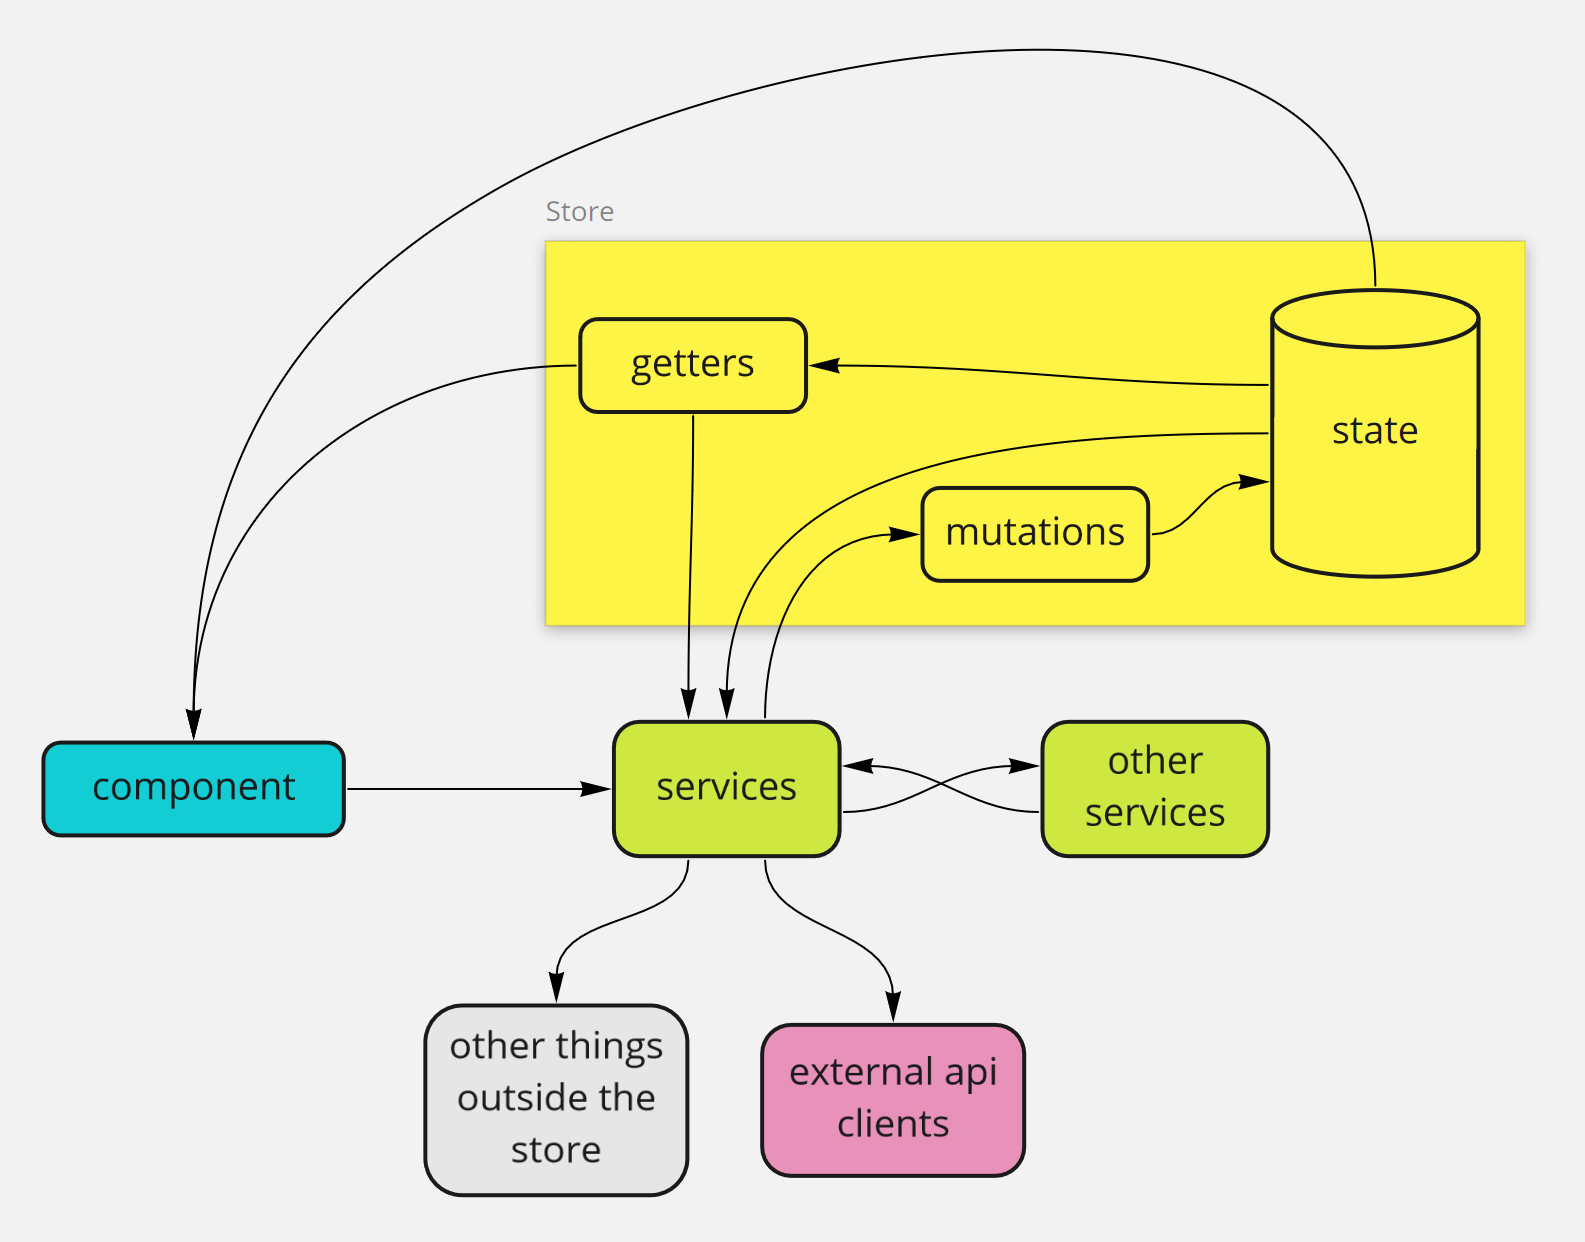
\includegraphics[width=0.7\textwidth]{Images/store.png}
\end{figure}
https://javascript.plainenglish.io/stop-using-actions-in-vuex-a14e23a7b0e6

Finisci di scrivere...

\section{Centralina}
Implementazione centralina


\section{Prodotto Finale}
\label{prodottofinale}
Il prodotto finale ha subito delle evoluzioni rispetto al mockup ma segue le linee
guida imposte.
TODO: Screen di esempio dell'applicazione
    % -*- root: ../main.tex -*-

% Esporre lo stato di funzionamento effettivo del sistema progettato ad elaborato concluso. Per ciascuna delle funzionalità salienti devono essere tabellate e discusse le performance riscontrate mediante opportuni test eseguiti in fase di validazione del progetto. I tempi di esecuzione/comunicazione devono essere accompagnati dalle caratteristiche dell'hardware sul quale è eseguito il software. Qualora l'elaborato includa algoritmi innovativi, indicarne la complessità computazionale (avendo cura di esporre lo pseudo codice nella sezione Implementazione).

\chapter{Testing e Performance}

Lo sviluppo delle applicazioni web a livello professionale richiede la qualità e la robustezza del codice che è stato prodotto. Per avere delle metriche concrete sulla qualità
del prodotto, è necessario coprire il progetto di test, sia automatici che manuali

\section{Unit Test}
Le parti più importanti della logica di business sono stati testati con gli unit test per migliorarne la robustezza e l'affidabilità
 \subsection{Backend}
 Il backend utilizza lo testing stack Mocha + Chai + Sinon. 
Mocha è il framework testing ricco e semplice che consente di creare facilmente
gli unit test eloquenti.
Chai è una libreria di assertions BDD/TDD che consente di creare le asserzioni
multi-paradigma per i test. Tali asserzioni rendono i tests più leggibili e forniscono messaggi di errore migliori in caso di errori. 
Sinon è la libreria per creare e gestire i test spies, stubs e mocks da utilizzare
negli unit test. Nel nostro caso è stato utilizzato soltanto per simulare l'invio delle email.

Durante lo sviluppo del backend è stata adoperata una collection Postman per testare tutte le varie chiamate al server. 

    % -*- root: ../main.tex -*-

% In questa sezione va discussa, eventualmente con l'ausilio di opportuni diagrammi (componenti, deployment), l'evoluzione del progetto presentato immaginando che venga adottato su larga scala. I dettagli qui esposti devono quindi astrarre dalle specifiche dell'elaborato qualora l'implementazione sia stata focalizzata su uno scenario isolato. A titolo d'esempio, qualora applicabile, devono essere evidenziate le criticità che si potrebbero incontrare e devono essere proposte soluzioni tipiche in contesti di cloud architecture per garantire un'adeguata resilienza, in termini di availability e scalability del sistema.

\chapter{Analisi di Deployment}

    % -*- root: ../main.tex -*-

%  piano di lavoro adottato. A tal fine, per ogni attività svolta durante la preparazione dell'elaborato (ad esempio: studio di una tecnologia, progettazione di un componente, implementazione di un algoritmo ecc. . . ) deve essere chiarita la collocazione temporale e devono essere indicate le risorse impiegate per svolgerla (giorni/uomo). I candidati possono ricorrere a opportuni diagrammi come quello di Gantt.

\chapter{Piano di lavoro}
Il lavoro è stato svolto utilizzando un approccio Scrum, con sprint periodici, di cui uno iniziale incentrato sullo studio delle tecnologie. Un diagramma di Gantt è stato creato all'inizio del progetto per definirne le tempistiche. Inizialmente una buona dose di tempo è stata impiegata per un design dettagliato, per non incorrere in cambiamenti in corso d'opera. Inoltre, si è prestata attenzione a costruire la relazione e la documentazione passo passo durante il lavoro. Qui di seguito viene riportato lo schema realizzato inizialmente. 
\begin{figure}[H]
    \caption{Gantt Chart Programmato}
    \label{fig:Gantt}
    \centering
    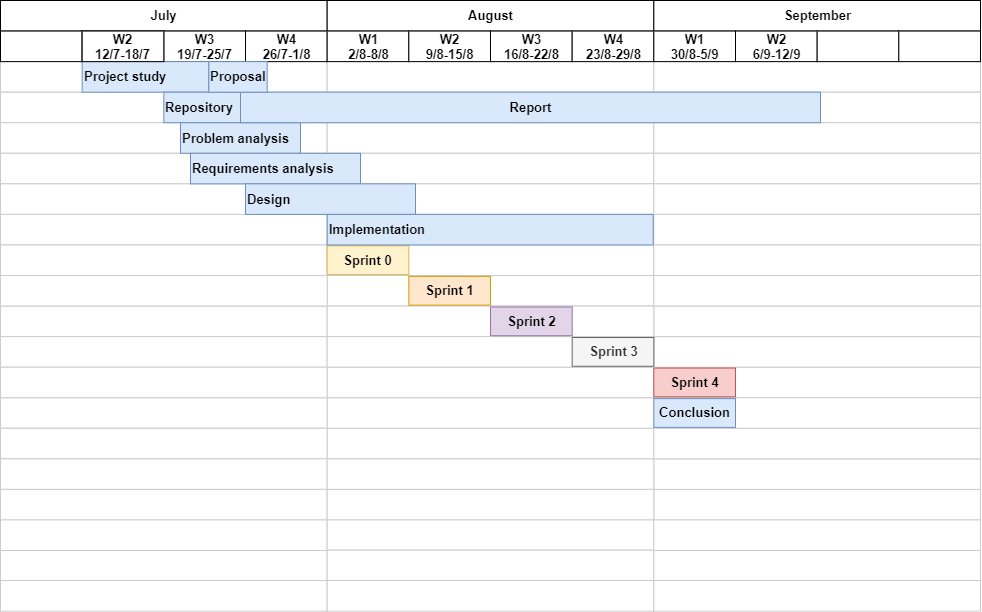
\includegraphics[width=1\textwidth]{DrawIo/GanttChart.png}
\end{figure}

Nonostante il programma dettagliato e le deadlines periodiche il progetto verso la fine si è dilazionato nel tempo. Lo si può vedere chiaramente dalla curva formata dal grafico. Riteniamo però che l'allungamento tempi sia dovuto anche a fattori esterni, quali l'inizio delle lezioni e il sovrapporsi di impegni non programmati. Di seguito è riportato il reale andamento del progetto nel tempo. 
\begin{figure}[H]
    \caption{Gantt Chart Reale}
    \label{fig:GanttReal}
    \centering
    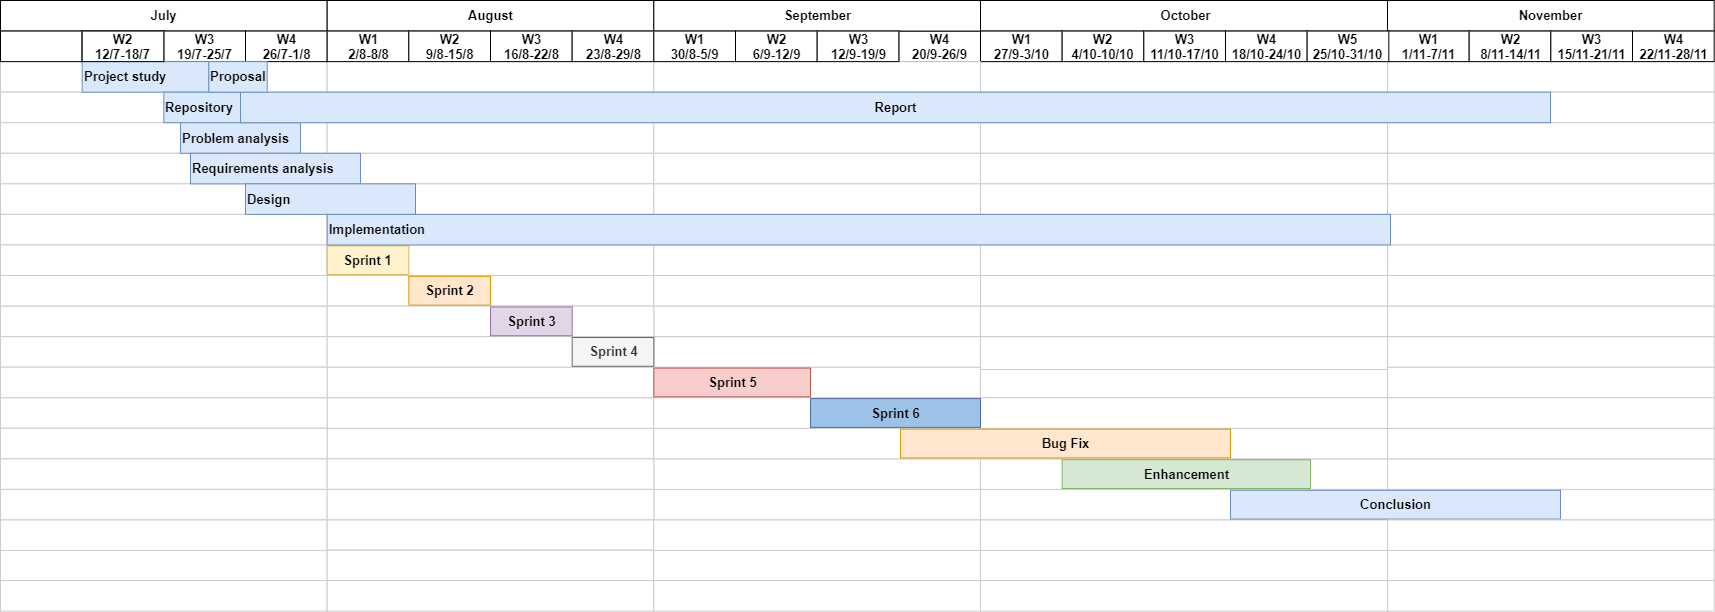
\includegraphics[width=1\textwidth]{DrawIo/GanttChartReal.png}
\end{figure}

\section{Sprints}

\subsection{Svolgimento}
Gli sprint sono stati portati avanti nel seguente modo:
    \paragraph{Sprint Planning}
        Pianificazione a inizio sprint degli obiettivi, tempistiche e responsabilità nel periodo dello sprint corrente. Diviso in due parti:
        \begin{itemize}
        \item\textbf{parte 1} 
            Viene raffinato e rivisto il product backlog, viene effettuata la scelta dello sprint goal (what).
        \item\textbf{parte 2}
            Si decidono gli item e viene raffinato come implementarli (how). Effettuato con solo il team senza la figura del product owner
        \end{itemize}
    \paragraph{[Iterativo] Daily scrum} Breve meeting svolto giornalmente. Viene utilizzato per gli aggiornamenti sull'andamento del progetto, senza scendere nei dettagli implementativi.
    \paragraph{[Occasionale] Pair Programming } Utilizzato per risolvere problemi che causano il blocco di un componente del team per parecchio tempo su una issue.
    \paragraph{Meeting finale}
        Riflessioni e considerazioni finali sullo spint passato. Suggerimenti per migliorare il prossimo. Diviso in tre parti: 
        \begin{itemize}
        \item\textbf{Product backlog refinement} aggiunta di dettagli e riordino del product backlog
        \item\textbf{Sprint review} è stato ispezionato l'incremento, il Minimum Viable Product o di risultati sul processo. Discernere cosa è stato fatto e cosa no
        \item\textbf{Retrospettiva} Considerazioni sul team stesso e sui miglioramenti per il prossimo sprint. 
        \end{itemize}
        
        

\subsection{Sprint 0}
All'interno dello sprint 0 il focus è stato ...
\paragraph{Deliverables} 
\begin{itemize}
    \item architettura base server
    \item scheletro relazione
\end{itemize}



    % -*- root: ../main.tex -*-
\chapter{Sprints}

\section{Svolgimento}
Gli sprint sono stati portati avanti nel seguente modo:
    \paragraph{Sprint Planning}
        Pianificazione a inizio sprint degli obiettivi, tempistiche e responsabilità nel periodo dello sprint corrente. Diviso in due parti:
        \begin{itemize}
        \item\textbf{parte 1} 
            Viene raffinato e rivisto il product backlog, viene effettuata la scelta dello sprint goal (what).
        \item\textbf{parte 2}
            Si decidono gli item e viene raffinato come implementarli (how). Effettuato con solo il team senza la figura del product owner
        \end{itemize}
    \paragraph{[Iterativo] Daily scrum} Breve meeting svolto giornalmente. Viene utilizzato per gli aggiornamenti sull'andamento del progetto, senza scendere nei dettagli implementativi.
    \paragraph{[Occasionale] Pair Programming } Utilizzato per risolvere problemi che causano il blocco di un componente del team per parecchio tempo su una issue.
    \paragraph{Meeting finale}
        Riflessioni e considerazioni finali sullo spint passato. Suggerimenti per migliorare il prossimo. Diviso in tre parti: 
        \begin{itemize}
        \item\textbf{Product backlog refinement} aggiunta di dettagli e riordino del product backlog
        \item\textbf{Sprint review} è stato ispezionato l'incremento, il Minimum Viable Product o di risultati sul processo. Discernere cosa è stato fatto e cosa no
        \item\textbf{Retrospettiva} Considerazioni sul team stesso e sui miglioramenti per il prossimo sprint. 
        \end{itemize}
        
        

\section{Sprint 0}
All'interno dello sprint 0 il focus è stato ...
\paragraph{Deliverables} 
\begin{itemize}
    \item architettura base server
    \item scheletro relazione
\end{itemize}



    % -*- root: ../main.tex -*-

\chapter{Conclusioni}
    \section{Commenti Finali}
        \subsection{Daniele Tentoni}
        \subsection{Silvia Zandoli}
        \subsection{Igor Lirussi}
        Al termine del percorso di sviluppo del progetto ritengo di aver acquisito una discreta moltitudine di nuove conoscenze. Sono state impiegate e integrate diverse tecnologie e metodologie anche complesse con cui sono state affinate parecchio le mie competenze nell'ambito. Sicuramente c'è ancora spazio per approfondire molti argomenti, ma nel complesso reputo sia servito a formare una base di conoscenza a tutto tondo. Il lavoro di gruppo ha permesso, infatti, di scambiarci nozioni a vicenda e ne sono più che contento, seppur mi rincresce non essere stato presente a volte come avrei voluto. Molte tecnologie usate sono state per me una scoperte \emph{in-itinere}, in quanto completamente nuove. Ritengo comunque il progetto sia stato particolarmente ambizioso e il risultato ottenuto a mio parere è più che soddisfacente. Infine, spero questo lavoro possa rappresentare una buona base di partenza per un eventuale sviluppo futuro. 
    \section{Sviluppi Futuri}
    In futuro, il progetto potrà essere migliorato nelle sue parti lasciando spazio a nuove tecnologie e, auspicabilmente, anche ad una commercializzazione. 
    Le aggiunte che abbiamo individuato sono sia di natura grafica che funzionale, ma, a causa delle tempistiche ridotte e del carico di lavoro, sono state demandate ad un'implementazione futura. \newline
    Eventualmente la parte funzionale si può estendere creando  nuove pagine per l'utente finale, con sezioni quali "notizie", "video degli utenti", "allerte meteo". Inoltre nuove funzioni possono sempre essere aggiunte al back-end per migliorare la parte di aggregazione delle varie previsioni con machine learning, ponderamento in base ai feedback o allo storico delle condizioni meteo reali. Può essere implementata una parte amministrativa del sito e integrata in maniera non invasiva della pubblicità. \newline
    La parte grafica invece può essere ulteriormente migliorata con animazioni e elementi accattivanti, eventualmente che rispecchino le attuali condizioni meteo. Inoltre mappe interattive possono aiutare l'utente ad avere un'idea più chiara della situazione geografica. Eventualmente anche temi personalizzati possono essere sviluppati per rispecchiare i gusti degli utilizzatori.  \newline
    Negli sviluppi futuri includiamo anche un interfacciamento con i social maggiormente diffusi, oramai essenziali allo sviluppo di un business. In questo modo si potrebbe automatizzare la creazione di post, facilitare l'interazione tra gli utenti, lo sviluppo di una community e l'esposizione della piattaforma.  \newline
    Inoltre, come possibili spin-off sono state individuate delle aree tematiche spesso ignorate in cui le previsioni sono necessarie, ad esempio previsioni per lo sport, quali venti per i praticanti di parapendio o correnti marine per i surfisti. Anche qui è altamente necessario l'utilizzo di device IoT.  \newline
    A riguardo, in futuro si potrebbe pensare ad una commercializzazione di un device integrato "ready to use" per delle previsioni più personali.  \newline
    In conclusione in futuro il progetto offre numerose opportunità di ampliamento, con interessanti prospettive sia dal lato tecnologico che dal lato business.  
    



\nocite{*} % Includes all references from the `references.bib` file
\printbibliography[title={Bibliografia completa}]

\end{document}
